\graphicspath{{02-TOF/Figures/}}

\newcommand{\Tzero}{\ensuremath{T0}}
\newcommand{\Gauss}{\ensuremath{\text{G}}}
\newcommand{\DT}{\ensuremath{\Delta T}}
\newcommand{\us}{\ensuremath{\mu\text{s}}}

\section{Time-of-flight detectors}
\label{Sect:TOF}

Three scintillator hodoscopes were used to measure the time of flight
(TOF) of the particles that made up the beam, the transverse position
at which the particle crossed each of the detectors, and to provide
the trigger for the experiment. 
TOF0 and TOF1~\cite{NOTE145,NOTE241,2010NIMPA.615...14B} were
placed upstream of the magnetic channel, while and TOF2~\cite{NOTE286}
was located downstream of the channel, mounted in front of the KL
pre-shower detector (see figure~\ref{fig:BL}).
The range of particle momentum delivered to the experiment was
determined by the settings of the two dipole magnets D1 and D2.
At 240\,MeV/$c$, the difference in the TOF for a muon and a
pion between TOF0 and TOF1 was about 1.3\,ns.
The system was therefore designed to measure the TOF with a
precision of 100\,ps. 
This allowed the TOF between the first pair of TOF stations 
to be used to discriminate between pions, muons, and electrons
contained within the beam with near 100\% efficiency~\cite{2016JInst..11P3001A}.
In addition, by assuming a particular mass for each particle, the
TOF measurement was used to infer the particle
momentum.
The TOF detectors operated smoothly during the running periods and
were essential for all the measurements that were
performed~\cite{Bogomilov:2012sr,Adams:2013lba,2015JInst..10P2012A,2016JInst..11P3001A,Adams:2018qhj,Bogomilov:2019kfj}.
\begin{figure}
  \begin{center}
    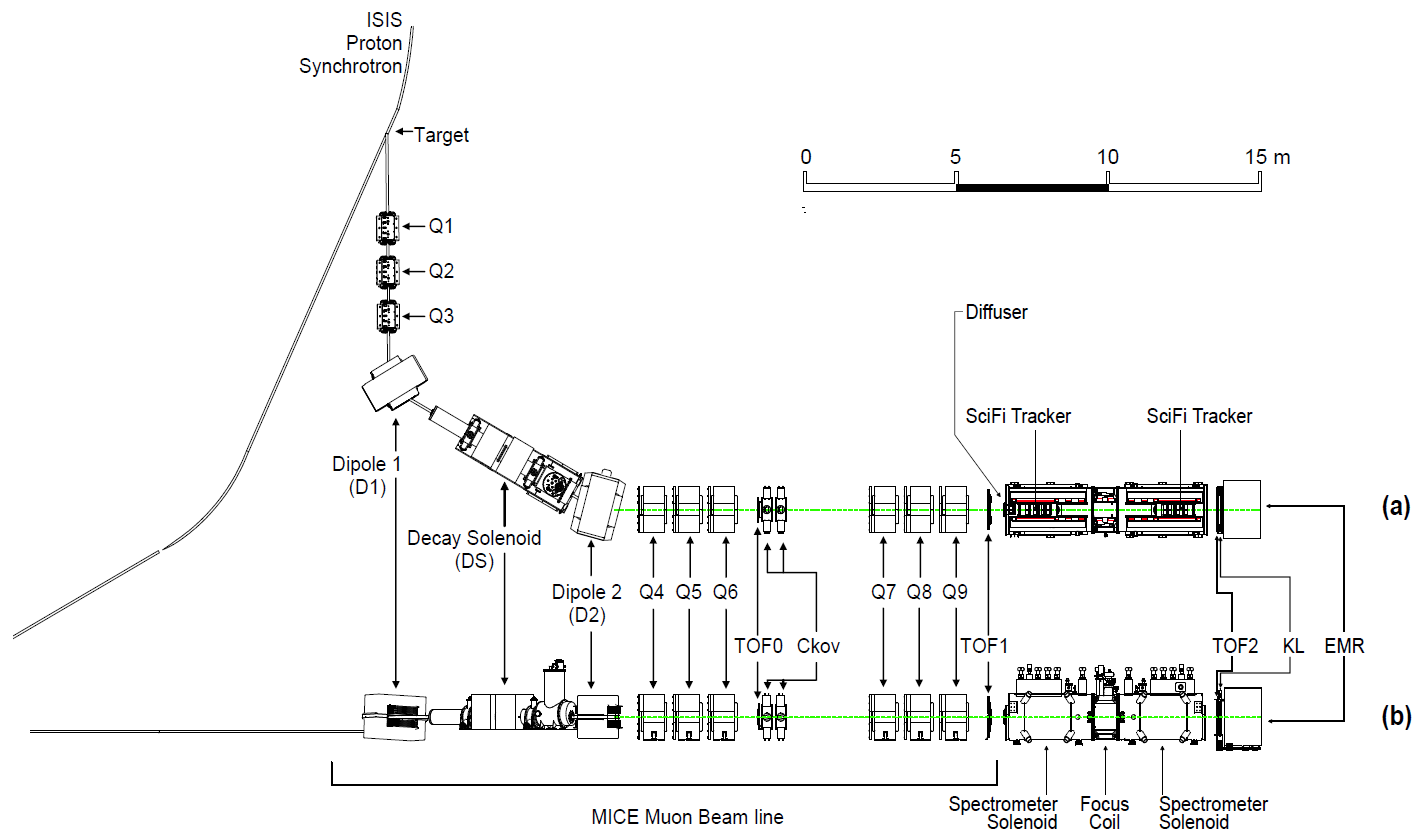
\includegraphics[width=1.0\columnwidth]{BL.png}
    \caption{
      MICE, top (a) and side (b) views, showing the full beam line
      starting from the target position on the proton synchrotron with the quadrupoles and dipoles (Q1 to Q9, D1, D2), the
      Decay Solenoid, and instrumented magnetic channel elements
      (including the trackers upstream and downstream of the cooling
      channel, placed inside superconducting solenoids) with all the
      other PID detectors (three TOF stations, two Ckov detectors, KL and
      the EMR).
      The cooling channel, defined by the liquid-hydrogen absorber
      vessel inside the Focus Coil, is shown in
      figure~\ref{Fig:AbsorberVessel:Diag}.
    }
    \label{fig:BL}
  \end{center}
\end{figure}

Each TOF station was made of two planes of 1\,inch thick scintillator
bars oriented along the $x$ and $y$ directions. 
The bars were made of BC-404 plastic scintillator.
A simple fishtail light-guide was used to attach each end of each bar
to R4998 Hamamatsu fast photomultiplier tubes (PMTs).
Each PMT was enclosed in an assembly that included the voltage divider
chain and a 1\,mm thick $\mu$-metal shield.
The shield was required to reduce the stray magnetic field within the
PMT to a negligible level~\cite{2010NIMPA.615...14B}.
To increase the count-rate stability, active dividers were used.
The TOF detector is illustrated in figure~\ref{fig:tof:schematic}.
\begin{figure}[!htb]
  \begin{center}
    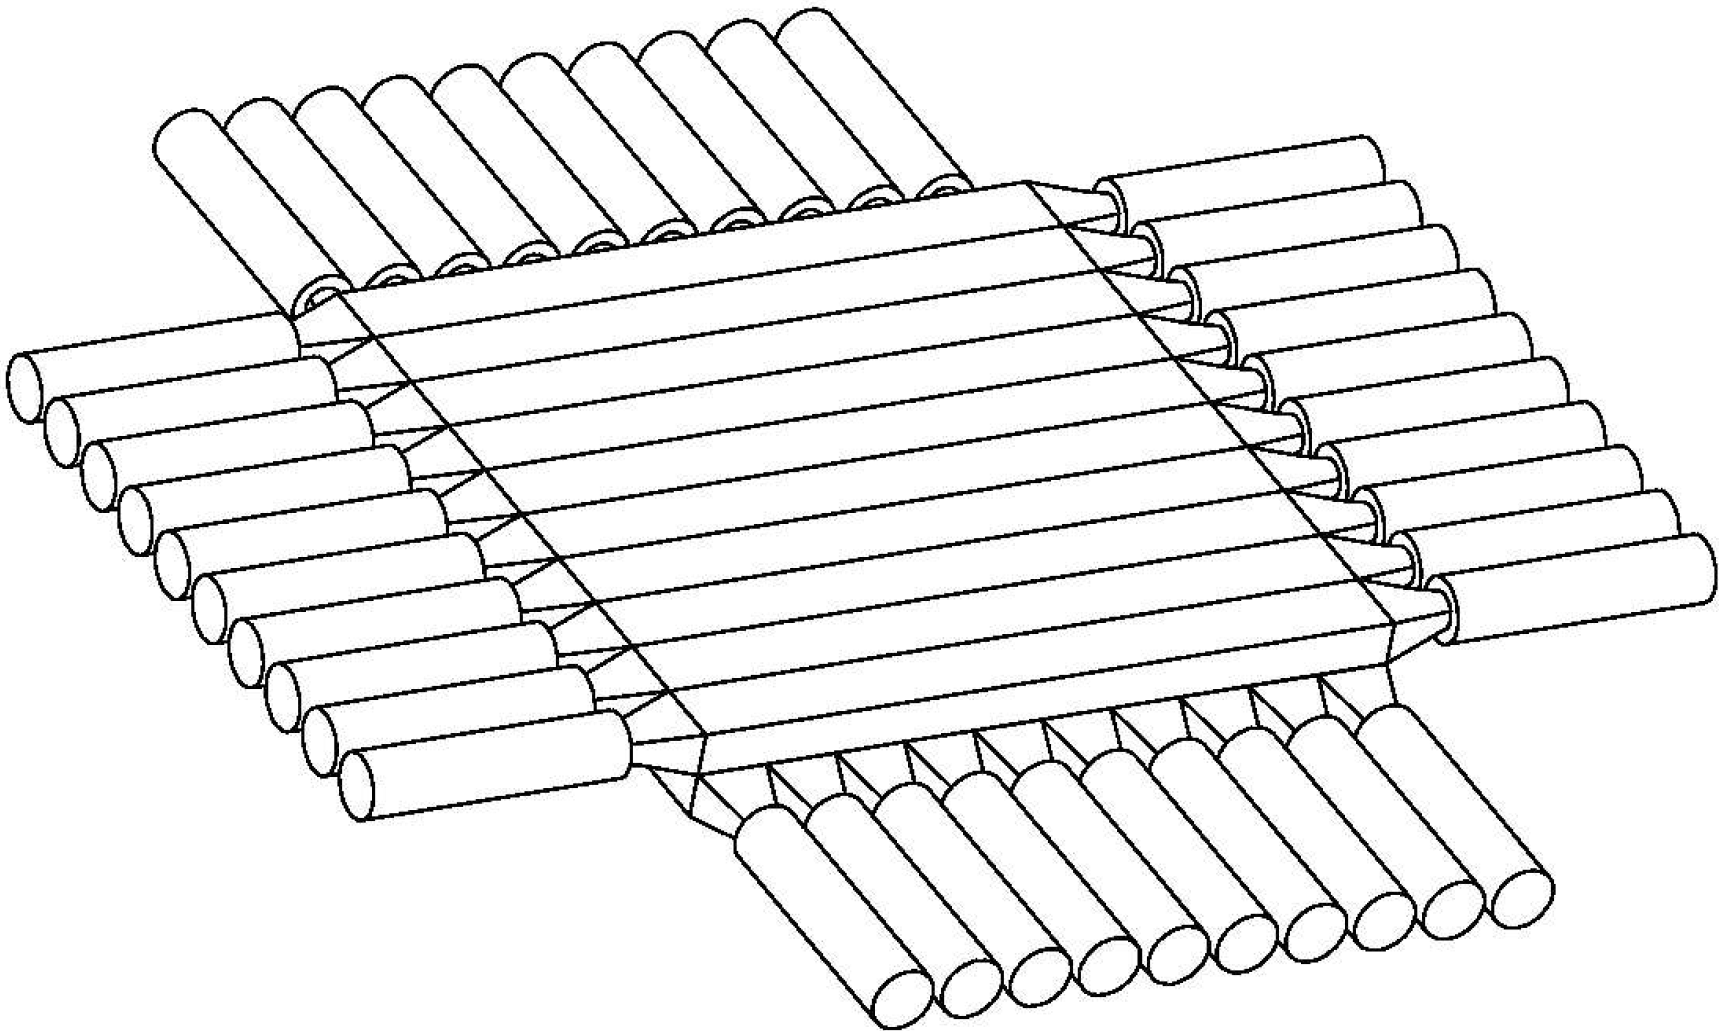
\includegraphics[width=8cm]{tof_diagram2}
    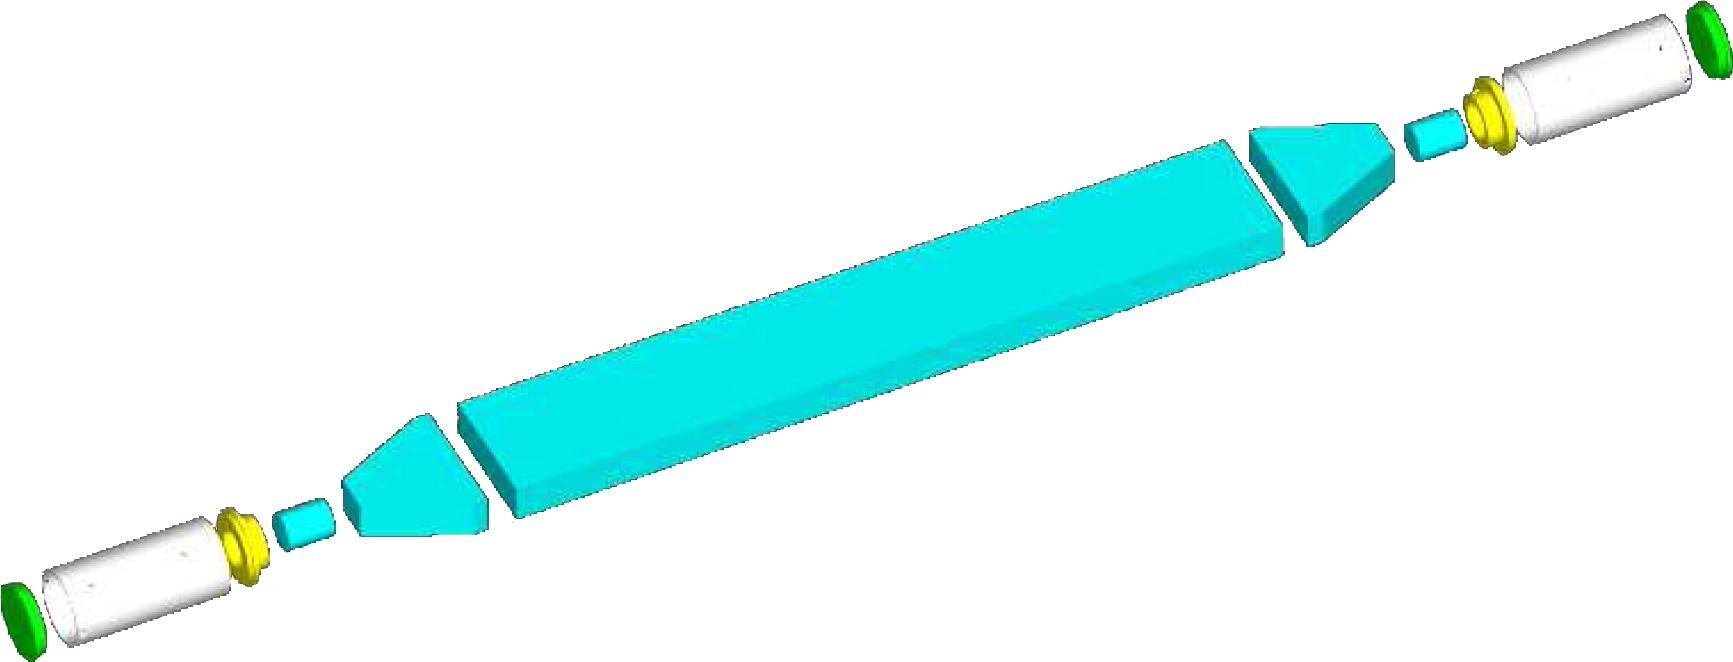
\includegraphics[height=3cm]{slab_design2}
  \end{center}
  \caption{
    The structure of the time-of-flight
    detectors~\cite{2010NIMPA.615...14B,NOTE145} showing the
    horizontal and vertical layers of slabs (left) and an exploded
    view of each slab (right). 
    The components of each slab are the central scintillator bar, two
    fishtail, clear plastic light-guides coupled to clear plastic
    matching pieces, and two PMTs.
  }
  \label{fig:tof:schematic}
\end{figure}

The active areas of the three hodoscopes are 40$\times$40\,cm$^2$
(TOF0), 42$\times$42\,cm$^2$ (TOF1), and 60$\times$60\,cm$^2$ (TOF2).
Each of the planes in TOF0 and TOF2 had 10 slabs while those in TOF1 had 7.
A passive splitter was used to take the signal from each of the PMTs
to: a CAMAC Lecroy 4115 leading-edge discriminator followed by a CAEN
V1290 TDC for time measurement; and to a CAEN V1724 FADC for
pulse-height measurement.
A local readout trigger was issued if the signals from each of the two
PMTs on a single slab crossed a specific threshold and overlapped.
TOF1 was used to trigger the readout of the experiment for most of the
data taking. \\

\noindent\textbf{Calibration} \\
\noindent
The intensity of the scintillation light produced when a particle
crossed the plastic scintillator rose rapidly, subsequently decaying
with a characteristic time of 1.8\,ns. 
The scintillation light travels from the particle-crossing point to
each end of the scintillator slab.
The light-travel time depends on the distance of the particle
crossing from the PMT.
The light-propagation speed in the slabs was determined to be 13.5\,cm/ns.

The local readout-trigger signal was distributed to all TDC boards and was
used as the reference time.
The time between a particle hit in a TOF slab and the time when the
trigger is generated varies with the position of the hit along the slab.
As a consequence, the reference time had an offset dependent on
the crossing position, an effect referred to as the
readout-trigger signal delay.
To compensate for this, the final time measurement in each station was
an average of the times recorded for each channel above
threshold.

Further delay was introduced by the signal-transit time of each PMT
and of the cable that led the signal to the readout electronics.
These signal-transit times were unique for each individual readout
channel and were determined by dedicated measurements.
The use of a linear, leading-edge discriminator lead to a correlation
between the total charge in the pulse and the time at which the
discriminator fired.
This correlation, referred to as the time-walk, introduced a
systematic offset in the time recorded by the TDC dependent on the pulse
height. 

Precise determination of the TOF requires a calibration procedure that
allows channel-by-channel variations in the response of the system to
be accounted for.
The calibration procedure described in~\cite{NOTE251} accounted for
each of the effects identified above. \\

\noindent\textbf{Reconstruction} \\
\noindent
A particle crossing a TOF station passes through two orthogonal
slabs.
Signals from each PMT were corrected for time-walk, readout-trigger
signal delay, and the channel-specific delays.
The slab-crossing time was taken to be the average of the corrected
PMT times.
Two slabs were taken to have been produced by the passage of a
particle if their slab-crossing times were within a 4\,ns window.
These two \textit{matched} slabs were used to define a pixel of area given by the
width of the slabs.
The particle-crossing time was then determined as the average of the
slab times and the approximate position of the particle crossing was
refined using the PMT signals in the two orthogonal slabs. \\

\noindent\textbf{Performance} \\
\noindent
The difference, $\Delta T$, between the slab times for \textit{matched} slabs
was used to determine the intrinsic time resolution, $\sigma_T$ of the
TOF system.
Assuming that the intrinsic resolution is the same in each of the
planes that make up a particular TOF station, the $\Delta T$
resolution, $\sigma_{\Delta T}$ will be given by
$\sigma_{\Delta T}=2\sigma_T$.
Figure~\ref{fig:SlabDtAll} shows the distributions of $\Delta T$ for
TOF0, TOF1, and TOF2 for a representative set of data taken in 2018.
The RMS width of the distributions are 114\,ps, 126\,ps, and 108\,ps
for TOF0, TOF1, and TOF2 respectively.
The distributions are similar, and the RMS of each distribution is
consistent with the measured intrinsic resolution of approximately
60\,ps~\cite{2010NIMPA.615...14B}.
\begin{figure}
  \begin{center}
    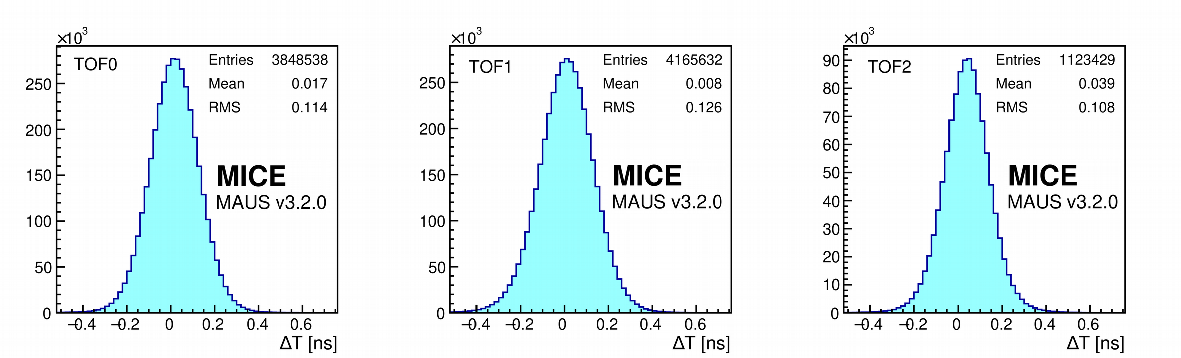
\includegraphics[width=0.9\columnwidth]{07_overall_slab_dt_edited.pdf}
  \end{center}
  \caption{
    Slab \DT{} distributions.
    Total width of the distribution was due to the resolution of
    individual pixels and due to the offsets in their \DT{}
    distributions.
  }
  \label{fig:SlabDtAll}
\end{figure}

Figure~\ref{fig:TOF_peaks} shows an example of distribution of the
measured TOF between TOF0 and TOF1.
The TOF peaks characteristic of electrons, muons, and pions are
clearly separated.
The width of the electron peak is approximately~0.10\,ns,
consistent with the spread calculated from a naive quadrature addition
of the timing resolution of the individual TOF stations.
\begin{figure}
  \begin{center}
    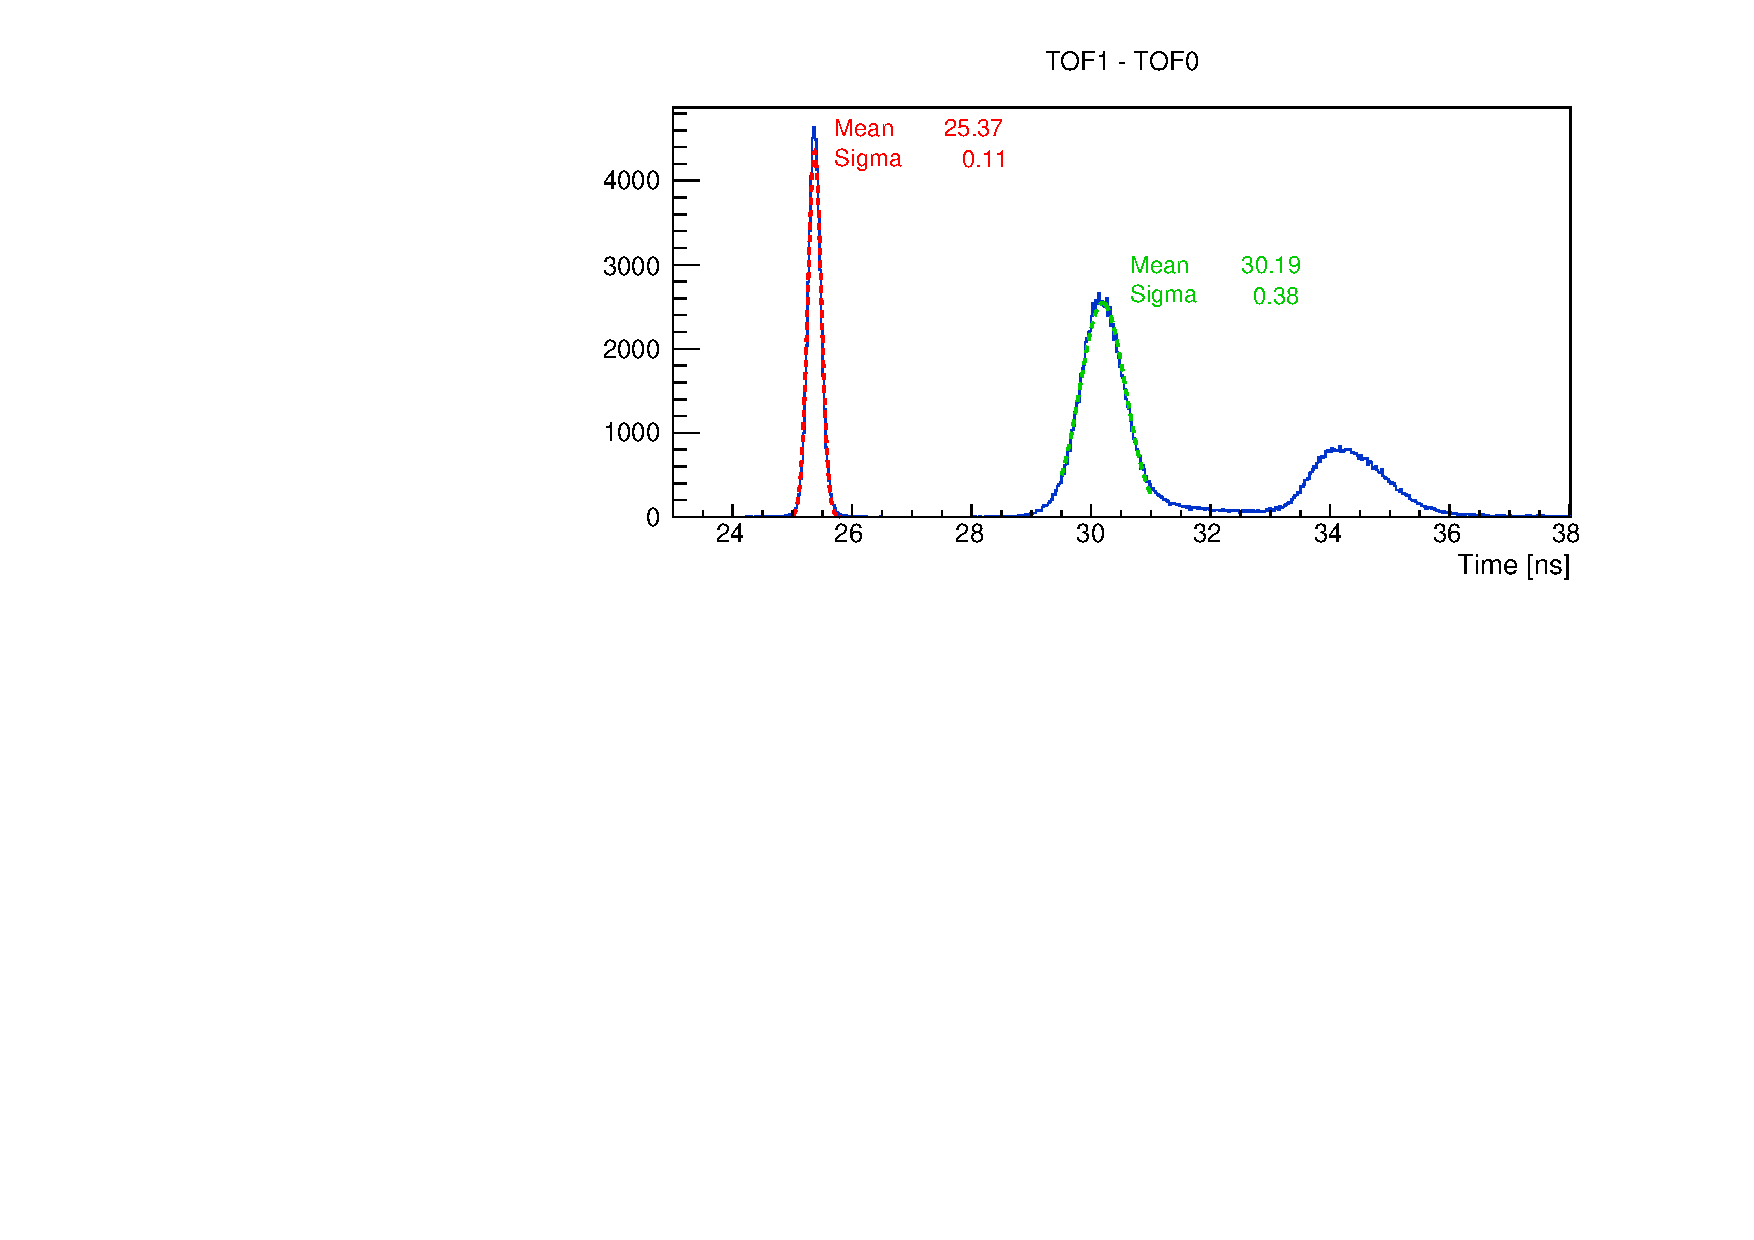
\includegraphics[width=0.6\columnwidth]{TOF_peaks.pdf}
  \end{center}
  \caption{
    Time of flight between TOF0 and TOF1 after all corrections have
    been applied. From the left: the well separated electron, muon and
    pion distributions.
  } 
  \label{fig:TOF_peaks}
\end{figure}
